\def\Ipe#1{\def\IPEfile{#1}\input{#1}}

\renewcommand{\Re}{{\rm I\!\hspace{-0.025em} R}}

\def\C{{\cal C}}
\def\G{{\cal G}}
\def\F{{\cal F}}
\def\I{{\cal I}}
\def\U{{\cal U}}
\def\M{{\cal M}}
\def\eps{{\varepsilon}}
\def\bd{{\partial}}
\def\dm{{\cal D}}

\chapter{2D Map Overlay} 
\label{I1_ChapterMapOverlay_2}

\section{Introduction}
\label{OVL_sec:example}

Given two planar subdivisions $S_1$ and $S_2$, the overlay of 
$S_1$ and $S_2$, denoted by $O(S_1,S_2)$ is the subdivision 
of the plane induced by the edges of $S_1$ and $S_2$.
In this case, $S_1$ and $S_2$ are called the {\em creators} 
of $O(S_1,S_2)$. The overlay of $S_1$ and $S_2$ is represented as the 
arrangement induced by $S_1$ and $S_2$ which maintains information 
regarding its creators, namely, every feature of $O(S_1,S_2)$ holds pointers 
to the respected features from $S_1$ and $S_2$ which caused its creation.
When a feature $f \in O(S_1,S_2)$ is contained in two other features 
$f_1 \in S_1$ and $f_2 \in S_2$, we say that $f_1$ and $f_2$ 
lay {\em above} $f$, alternatively, we say that 
$f$ is {\em below} $f_1$ and $f_2$.
Every feature in the overlay $O(S_1, S_2)$ maintains the 
information regarding the features from $S_1$ and $S_2$ laying above it.

The subdivision, representing the overlay and its two creators, 
can be either a {\it planar map} 
(see Chapter~\ref{I1_ChapterPlanarMap}) 
or a {\it planar map with intersections} 
(see Chapter~\ref{I1_ChapterPmwx}).
%or an {\it arrangement} (see Chapter~\ref{I1_ChapterArrangement_2}).

Figure~\ref{OVL_sec:overlay_example} displays an overlay of two given rectangles.

% \begin{figure}
%     \begin{center}
%         \ \psfig{figure=.overlay_example.ps,width=14cm} \
%     \end{center}
%     \vspace{-2ex}
%     \caption{Two rectangles (left) and their overlay (right). We denote the subdivision 
%        induced by the first rectangle by $S_1$ and the second by $S_2$. 
%        The face $f$ of the overlay is below $f_1$ and the unbounded face of $S_2$. 
%        The halfedge $e$ of the overlay contains a halfedge pointer to $e_2$ and two faces pointers 
%        to $f_1$ and to $f_2$. The vertex $v$ of the overlay points to $v_2$, contains a halfedge 
%        pointer to $e_2$ and is lying below $f_1$ and $f_2$.}
%     \label{OVL_sec:overlay_example}
% \end{figure}

% \begin{figure}[h]
% \begin{ccTexOnly}
%     \centerline{
%       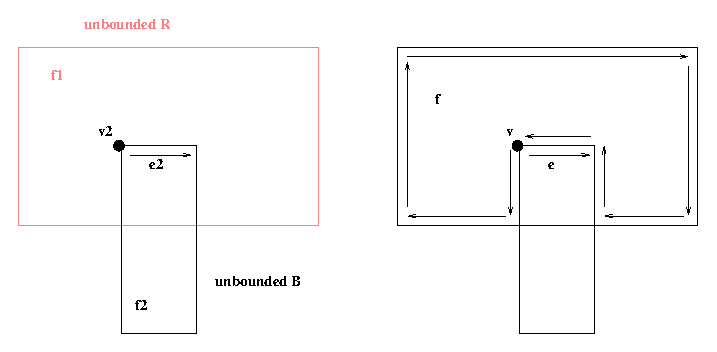
\includegraphics{overlay_example.ps}
%     }
% \end{ccTexOnly}

% \caption{Two rectangles (left) and their overlay (right). We denote the subdivision 
% induced by the first rectangle by $S_1$ and the second by $S_2$. 
% The face $f$ of the overlay is below $f_1$ and the unbounded face of $S_2$. 
% The halfedge $e$ of the overlay contains a halfedge pointer to $e_2$ and two faces pointers 
% to $f_1$ and to $f_2$. The vertex $v$ of the overlay points to $v_2$, contains a halfedge 
% pointer to $e_2$ and is lying below $f_1$ and $f_2$.
% \label{OVL_sec:overlay_example}}

\section{Software Design}
The \ccc{Map_overlay<Subdivision,Notifier>} class 
is a data structure for maintaining 2D map overlay.
The data structure maintains the subdivision obtained by overlaying 
the two creators,
and also contains two pointers to these creators. 
The underlying combinatorial structure is determined by the
(i) {\it Subdivision} which presents the subdivision type of the arrangement 
representing the overlay and its two creators. 
In our usage, {\it Subdivision} is a \ccc{Planar Map}, 
a \ccc{Planar Map With Intersections}.
% or an a \ccc{Arrangement}.
Notice that the choice of a subdivision type determines the choice 
of a DCEL and a traits class.
(ii) {\it Notifier>} is the notifier class used to update the overlay features. 
{\it Notifier} should be a model of the 
\ccc{PlanarMapWithIntersectionsChangeNotification_2} concept.

\paragraph{Map Overlay Algorithms:}
The input to our algorithms are two planar subdivisions denoted by $S_1$ and $S_2$ having 
$N$ vertices in total. The overlay of $S_1$ and $S_2$ has $N+k$ vertices, 
while $k$ is the number of intersections between 
$S_1$ and $S_2$. 
Consequentially, the combinatorial complexity of the overlay is quadratic 
in the size of $S_1$ and $S_2$ in the worst case.
We deviced and implementated two different algorithms for computing the map-overlay 
of two given planar subdivisions, 
which we refer to as the {\it incremental} algorithm and the {\it sweep-line} algorithm. 
In general, each of these algorithms constructs the overlay by inserting 
the curves of $S_1$ and $S_2$ into the subdivision representing the overlay,
and maintaining within each input curve its corresponding halfedge. 
The latter information is needed when using the notifier in order to
update the creator pointers. 

Our experimets show that the sweep-line algorithm is much faster than the incremental algorithm,
and hence, users are most encouraged to employ the sweep-line algorithm 
and use \ccc{Planar Map} as their subdivision. 

\paragraph{Map Overlay DCEL:}
The \ccc{Map_overlay_default_dcel<Traits,Vertex_base,Halfedge_base,Face_base>}
class is the data structure representing the DCEL of the overlay. 
The basic components of the DCEL of the overlay are built 
on top of the basic components of the \ccc{Planar Map} or the \ccc{Planar Map With Intersections} 
(depending on the subdivision we choose in order to represent the overlay and its 
two creators).

The additional information we maintain in these components is the pointers 
to the creator components.
Each feature of the overlay points to the features of the creartors above it.
This information is maintained in the basic components of the DCEL of the overlay, 
which implies that each face denoted by $f$ of $O(S_1, S_2)$ contains two pointers 
to the two faces of $S_1$ and $S_2$  above it. 
In the same way, each halfedge $e$ contains two pointers to the halfedges 
from $S_1$ and $S_2$ created it, note that we need two pointers in the case of overlapping curves. 
Each halfedge $e$ also maintains two pointers to the faces of the creators above it. 
Finally, each vertex $v$ of the DCEL of the overlay contains two pointers to the 
possibly two vertices of $S_1$ and $S_2$ above it, 
as well as two pointers to the possibly respected halfedges of $S_1$ and $S_2$ 
contain it, and in addition, $v$ contains two pointers to the 
faces of the creators above it. If $v$ is laying on the boundary of some faces of its creators, 
we choose one such face arbitrarily.

\paragraph{Map Overlay Notifier:}
Updating the DCEL additional attributes is performed by the {\em notifier} class.
We extend and override the notification functions of the basic {\em notifier}, defined 
in the \ccc{Planar_Map} package (see Chapter~\ref{I1_ChapterPlanarMap}), 
to update the corresponding features constructed by the overlay. 

The \ccc{Map_overlay_default_notifier<Subdivision>} class 
keeps on updating the additional information in the DCEL.
It updates the pointers to the components of the creators.
The notifier class overrides only the functions \ccStyle{add_edge} 
and \ccStyle{split_edge} of the basic notifier defined for \ccc{Planar_Map}.
In our implementation these functions update 
the pointers of the halfedges and the vertices in the DCEL 
presenting the overlay, see Chapter~\ref{I1_ChapterPlanarMap} for details.
In order to update the creator face pointers, we define a new function in our notifier, 
which traverses all features in the overlay in a DFS manner and updates the 
corresponding pointers. This function is invoked once we have terminated 
inserting into the overlay all the curves of $S_1$ and $S_2$.
We did not use the \ccStyle{split_face} function in order to update a face pointers, 
since it is invoked each time a cycle in the DCEL is closed and degrade performance. 

\subsection{Example of an Overlaying Two Subdivisions of Line Segments:}
The following example demonstrates a simple usage of the {\it Map Overlay} package.
In this example we construct two planar maps of line segments. 
Then we construct their overlay when using the sweep-line algorithm, which is 
the default algorithm for the overlay construction. 
After the overlay is constructed, we write its corresponding planar map to the 
standatd output stream. 

\ccIncludeExampleCode{Map_overlay_2/example1.C}
The input of the program is a text file containing two lists of segments, 
each of which represents an input subdivision.
\ccIncludeExampleCode{Map_overlay_2/example1.cin}

The output of the program looks like this:
\ccIncludeExampleCode{Map_overlay_2/example1.cout}
